\documentclass[11pt,a4paper]{article}

\usepackage[a4paper,margin=23mm,headheight=15pt]{geometry}
\usepackage[T1]{fontenc}
\usepackage{lmodern}
\usepackage{microtype}
\usepackage{graphicx}
\usepackage{booktabs}
\usepackage{tabularx}
\usepackage{array}
\usepackage{caption}
\usepackage{subcaption}
\usepackage{float}
\usepackage{amsmath}
\usepackage{xcolor}
\usepackage{titlesec}
\usepackage{fancyhdr}
\usepackage{hyperref}

\definecolor{UPESnavy}{HTML}{15345B}
\definecolor{UPESblue}{HTML}{2D6FA5}
\definecolor{LightBlue}{HTML}{EAF1F7}

\hypersetup{
  colorlinks=true,
  linkcolor=UPESblue,
  urlcolor=UPESblue,
  citecolor=UPESblue,
  pdftitle={Hotel Accounts Analysis},
  pdfauthor={Isha Vijay, Saranshi Chitra, Shaurya Singhal}
}

\titleformat{\section}
  {\Large\bfseries\color{UPESnavy}}{\thesection}{0.7em}{}
\titleformat{\subsection}
  {\large\bfseries\color{UPESblue}}{\thesubsection}{0.7em}{}
\titlespacing*{\section}{0pt}{1.2em}{0.4em}
\titlespacing*{\subsection}{0pt}{0.8em}{0.25em}

\setlength{\parindent}{0pt}
\setlength{\parskip}{0.38em}
\renewcommand{\arraystretch}{1.15}
\setlength{\emergencystretch}{2em}
\captionsetup{font=small,labelfont=bf}

\pagestyle{fancy}
\fancyhf{}
\lhead{\small\textcolor{UPESnavy}{Hotel Accounts Analysis}}
\rhead{\small\textcolor{UPESnavy}{Fundamentals of Data Science}}
\cfoot{\thepage}
\renewcommand{\headrulewidth}{0.4pt}

\newcommand{\INR}{INR~}
\newcommand{\sourcecaption}{\par\smallskip{\footnotesize\textit{Source: Figure reproduced from the supplied project report.}}}

\begin{document}

\pagenumbering{roman}
\begin{titlepage}
  \thispagestyle{empty}
  \centering
  \vspace*{10mm}
  
\includegraphics[width=2.4in]{figures/upes_logo.jpeg}

  \vspace{17mm}
  {\Large\textcolor{UPESblue}{FUNDAMENTALS OF DATA SCIENCE}\par}
  \vspace{6mm}
  {\huge\bfseries\textcolor{UPESnavy}{Hotel Accounts Analysis}\par}
  \vspace{4mm}
  {\Large Data Cleaning, Statistical Analysis and Prediction\par}

  \vspace{14mm}
  {\large Technical Project Report\par}
  \vspace{3mm}
  {\normalsize Dataset period: 1--20 April 2025\par}

  \vfill
  \begin{minipage}{0.8\textwidth}
    \centering
    \textbf{Submitted by}\par
    Isha Vijay \quad (590027876)\\
    Saranshi Chitra \quad (590027413)\\
    Shaurya Singhal \quad (590023883)

    \vspace{7mm}
    \textbf{Submitted to}\par
    Virendra Kadyan
  \end{minipage}
  \vspace{10mm}
\end{titlepage}
\pagenumbering{arabic}

\section{Problem identification and objectives}
Hotel managers need consistent records to understand revenue, operating expenses, tax amounts and transaction patterns across departments. Ledger errors can hide the correct amount or make departmental comparisons unreliable. This project uses a small hotel accounts dataset to demonstrate data cleaning, exploratory analysis, statistical tests, dimensionality reduction, classification and regression.

The project objectives are to:
\begin{enumerate}
  \item validate and clean the transaction ledger while recording each decision;
  \item summarize revenue, expenses and GST, and compare transaction groups;
  \item use hypothesis tests to examine differences and categorical relationships;
  \item use PCA to summarize the numeric features;
  \item use LDA to classify revenue and expense transactions;
  \item fit a regression model for transaction amount and interpret its limits.
\end{enumerate}

The scope is 100 transactions from one hotel over 20 days in April 2025. The data has no occupancy, customer-level or multi-month information, so the project does not estimate annual performance or establish real-world causal effects.

\section{Data collection and understanding}
This report follows the supplied project assessment criteria \cite{rubric}. The supplied workbook contains 100 records and 18 original fields. The analysis-ready sheet has 29 columns after derived and encoded fields were added. The accompanying data description identifies the records as secondary and generated; no external collection source is documented \cite{dataset,description}.

\begin{table}[H]
\centering
\caption{Main dataset attributes and their roles}
\small
\begin{tabularx}{\textwidth}{>{\raggedright\arraybackslash}p{0.25\textwidth}>{\raggedright\arraybackslash}p{0.24\textwidth}X}
\toprule
Attribute group & Type & Examples and use\\
\midrule
Identifiers & Text, not measurements & Transaction ID, voucher and reference numbers; used to identify records only.\\
Date & Date and elapsed time & Transaction date and day index; used for the daily trend and regression.\\
Categories & Nominal & Department, transaction type, account head, payment mode, cost center and approval status.\\
Amounts & Continuous numeric & Debit, credit, transaction amount, net amount and GST amount, all in INR.\\
Rates and codes & Numeric or coded category & GST rate is stored as a fraction; account code is a category even though it looks numeric.\\
\bottomrule
\end{tabularx}
\end{table}

There are eight departments, 12 account heads and five payment modes. Sixty records are revenue receipts and 40 are operating expenses. Five transactions are recorded per day. The transaction amount used in the analysis is debit plus credit. Net amount is a signed value calculated as credit minus debit \cite{dataset,description}.

\clearpage
\section{Data preprocessing and cleaning}
The analysis-ready workbook was checked before statistical analysis. The decisions below preserve the original records while using corrected values where needed \cite{projectreport,dataset}.

\begin{table}[H]
\centering
\caption{Data quality checks and actions}
\small
\begin{tabularx}{\textwidth}{>{\raggedright\arraybackslash}p{0.2\textwidth}>{\raggedright\arraybackslash}p{0.34\textwidth}X}
\toprule
Check & Finding & Action\\
\midrule
Missing values & No missing values in the analysis-ready workbook. & No imputation was needed.\\
Duplicates & No duplicate rows, transaction IDs or voucher numbers. & No records were removed.\\
Net amount & 17 original values (IDs 0084--0100) were zero despite a non-zero debit or credit. & Recalculated net amount as credit minus debit; kept the original column for comparison.\\
GST & Ten records have a zero GST rate; recalculated GST matches the original GST amount. & Kept zero-rate rows and treated them as exempt or possibly missing for interpretation.\\
Department coding & Some entries pair an account head with an unrelated department. & Kept the source entries; used account head for account-level analysis.\\
Data types & Date values and GST rates needed consistent interpretation. & Converted dates to date values and retained GST rate as a fraction.\\
Outliers & No transaction amount exceeded the reported IQR fences; maximum was INR 16,089. & No values were removed as outliers.\\
\bottomrule
\end{tabularx}
\end{table}

\section{Exploratory analysis and statistical implementation}
Analysis was performed in Python using pandas, NumPy, SciPy, statsmodels and scikit-learn. The significance level was $\alpha=0.05$. Transaction amount is the sum of debit and credit; net amount and GST amount are computed separately:
\begin{align}
  A_i &= D_i + C_i, \\
  N_i &= C_i - D_i, \\
  G_i &= A_i r_i,
\end{align}
where $A_i$ is transaction amount, $D_i$ is debit, $C_i$ is credit and $r_i$ is the GST rate.

\subsection{Descriptive statistics}
Across all 100 transactions, mean amount was INR 8,235.9, median INR 8,074.5, standard deviation INR 3,982.8, minimum INR 1,474 and maximum INR 16,089. The reported skewness was 0.17, indicating a roughly symmetric sample distribution.

\begin{table}[H]
\centering
\caption{Transaction amount by transaction type}
\begin{tabularx}{0.9\textwidth}{>{\raggedright\arraybackslash}Xrrr}
\toprule
Group & Records & Mean (INR) & Total (INR)\\
\midrule
Revenue receipts & 60 & 9,444.5 & 566,670\\
Operating expenses & 40 & 6,423.0 & 256,920\\
All transactions & 100 & 8,235.9 & 823,590\\
\bottomrule
\end{tabularx}
\end{table}

\clearpage
\pagestyle{fancy}
\begin{samepage}
The four revenue heads are similar in total: Spa INR 146,805, Room INR 143,380, Restaurant INR 139,955 and Banquet INR 136,530. Laundry is the largest listed expense head at INR 37,414. The total revenue--expense difference in this sample is INR 309,750; it is not presented as hotel profit because the dataset is limited and generated.
\end{samepage}

\subsection{Hypothesis tests}
For two independent groups, the Welch statistic compares the sample means without requiring equal variances:
\begin{equation}
  t = \frac{\bar{x}_1-\bar{x}_2}
  {\sqrt{s_1^2/n_1+s_2^2/n_2}}.
\end{equation}
For one-way ANOVA, $F=MS_{between}/MS_{within}$. A chi-square test of independence uses
\begin{equation}
  \chi^2 = \sum_{i,j}\frac{(O_{ij}-E_{ij})^2}{E_{ij}},
\end{equation}
where $O_{ij}$ and $E_{ij}$ are observed and expected cell counts. These tests describe the sample and rely on the design and assumptions of each test.

\begin{table}[H]
\centering
\caption{Selected hypothesis test results}
\small
\begin{tabularx}{\textwidth}{>{\raggedright\arraybackslash}Xrr>{\raggedright\arraybackslash}p{0.34\textwidth}}
\toprule
Test & Statistic & $p$-value & Interpretation\\
\midrule
Revenue mean vs. INR 9,000 & One-sample $t=0.864$ & 0.391 & No significant difference from the assumed benchmark.\\
Revenue vs. expense mean & $t=3.986$ & 0.00013 & Mean transaction amounts differ.\\
Welch revenue vs. expense & $t=4.149$ & 0.00007 & Same conclusion without equal-variance assumption.\\
All amounts vs. INR 8,000 & One-sample $z=0.592$ & 0.554 & No significant difference from the assumed benchmark.\\
Revenue vs. expense & Two-sample $z=3.986$ & $<0.001$ & Approximate result using an estimated standard deviation.\\
Revenue account heads & $F=0.078$ & 0.972 & No evidence of different mean amounts.\\
Expense account heads & $F=0.286$ & 0.955 & No evidence of different mean amounts.\\
Departments & $F=0.118$ & 0.997 & No evidence of different mean amounts.\\
Payment modes & $F=3.869$ & 0.0059 & Difference is confounded with transaction type.\\
Transaction type vs. GST rate & $\chi^2=90.0$ & $<0.001$ & Strong association; Cramer's $V=0.95$.\\
\bottomrule
\end{tabularx}
\end{table}

The two-sample z-test agrees with the t-test, but its population standard deviation was estimated from the sample, so it is only an approximation. Payment mode is structurally linked to transaction type: some modes occur only for revenue and others only for expenses. Pending approval has only six records; the project therefore also reports Fisher's exact test ($p=1.0$). The GST test's minimum expected count is four, so its chi-square result should also be interpreted cautiously \cite{projectreport}.

\section{Data visualization and results}
The box plot shows higher typical transaction amounts for revenue receipts than for expenses, with spread in both groups. The daily totals rise across most of the period and drop on the final day. This pattern is consistent with the reported correlation of $r=0.84$ between day and transaction amount, but the short generated series is not a forecast of future hotel activity.

\begin{figure}[H]
\centering
\begin{subfigure}[t]{0.48\textwidth}
  \centering
  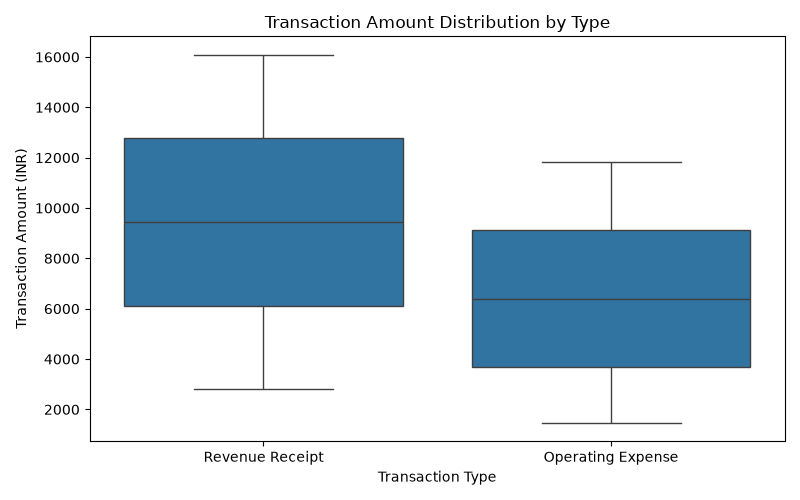
\includegraphics[width=\linewidth]{figures/transaction_amount_by_type.png}
  \caption{Amounts by transaction type}
\end{subfigure}\hfill
\begin{subfigure}[t]{0.48\textwidth}
  \centering
  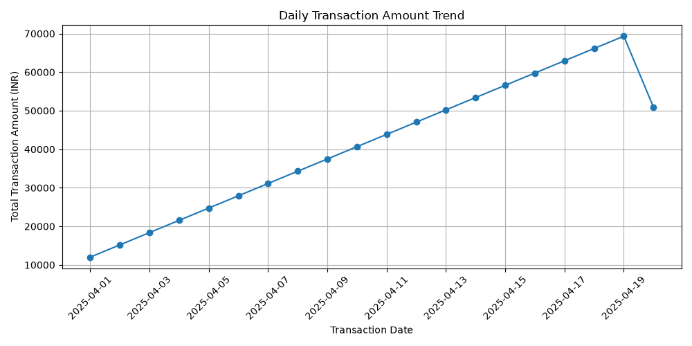
\includegraphics[width=\linewidth]{figures/daily_transaction_trend.png}
  \caption{Daily total amount}
\end{subfigure}
\caption{Exploratory views of hotel transaction amounts.}
\sourcecaption
\end{figure}

Amount and GST amount have a reported correlation of $r=0.74$. Correlations show association, not cause. The correlation heatmap summarizes selected numeric fields and should be read alongside the data definitions, particularly for coded categories.

\begin{figure}[H]
\centering
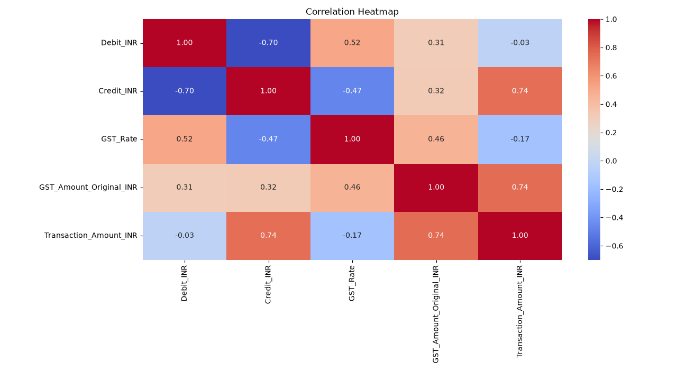
\includegraphics[width=0.77\textwidth]{figures/correlation_heatmap.png}
\caption{Correlation heatmap for selected numeric fields.}
\sourcecaption
\end{figure}

\section{Feature reduction and predictive models}
\subsection{Principal Component Analysis}
The project standardized five numeric features (amount, GST rate, GST amount, day and account code) and applied PCA. Standardization and the eigenvalue problem are:
\begin{equation}
  z_{ij}=\frac{x_{ij}-\mu_j}{\sigma_j},
  \qquad \Sigma v_k=\lambda_k v_k,
\end{equation}
where $\mu_j$ and $\sigma_j$ are the mean and standard deviation of feature $j$, and $\lambda_k$ is the variance explained by component $k$. PC1 explains 51.3\% and PC2 explains 33.9\%, for a cumulative 85.2\%. The project interprets PC1 as transaction scale and time, and PC2 as transaction type. Account code is categorical, despite its numeric appearance, so its PCA loading should not be read as a measured numeric effect.

\begin{figure}[H]
\centering
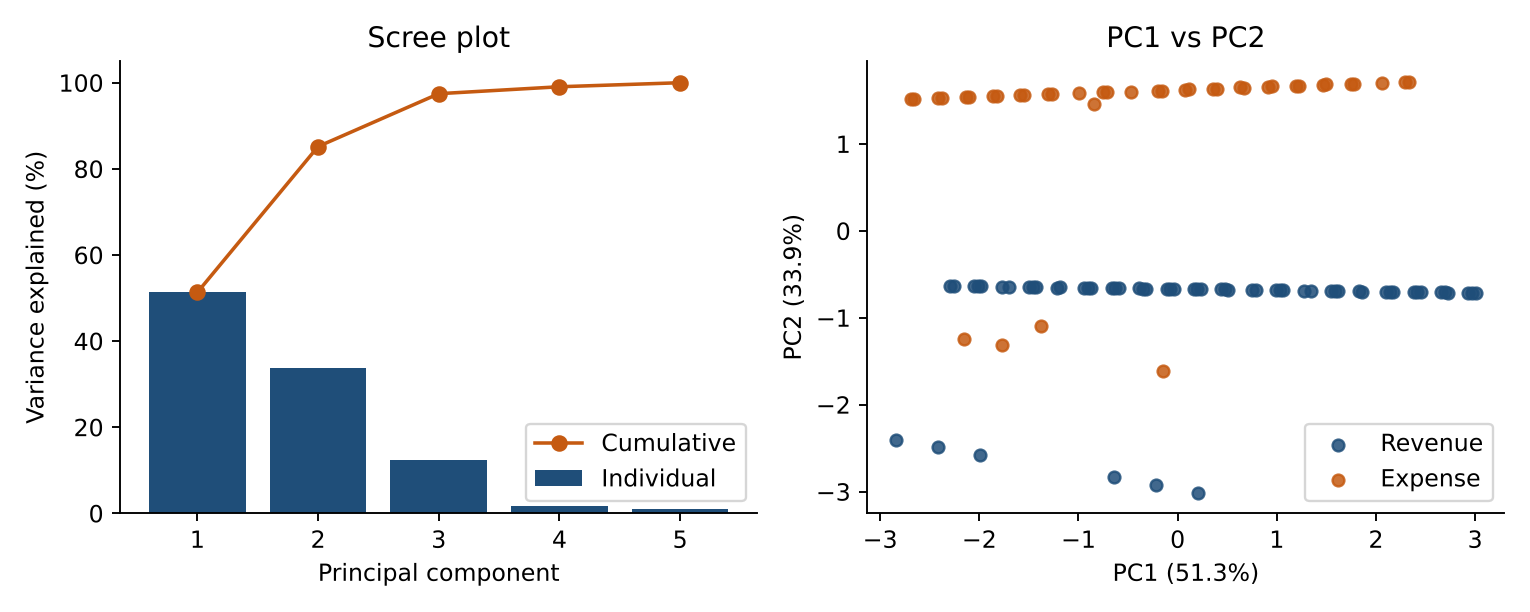
\includegraphics[width=0.88\textwidth]{figures/pca_variance_and_scores.png}
\caption{PCA scree plot and projection onto the first two components.}
\sourcecaption
\end{figure}

\subsection{Linear Discriminant Analysis}
LDA classifies records by finding a direction that separates groups. Its Fisher criterion is
\begin{equation}
  J(w)=\frac{w^{\mathsf T}S_Bw}{w^{\mathsf T}S_Ww},
\end{equation}
where $S_B$ and $S_W$ are between-class and within-class scatter matrices. The target was transaction type, using amount, GST rate, GST amount and day as features.

\begin{table}[H]
\centering
\caption{LDA training confusion matrix}
\begin{tabular}{lrr}
\toprule
Actual class & Predicted expense & Predicted revenue\\
\midrule
Expense & 37 & 3\\
Revenue & 0 & 60\\
\bottomrule
\end{tabular}
\end{table}

Training accuracy was 97\%, and reported five-fold cross-validated accuracy was 98\%. All three training errors were expenses predicted as revenue. GST features partly encode transaction type in this dataset, so the cross-validated score may overstate performance on new records.

\begin{figure}[H]
\centering
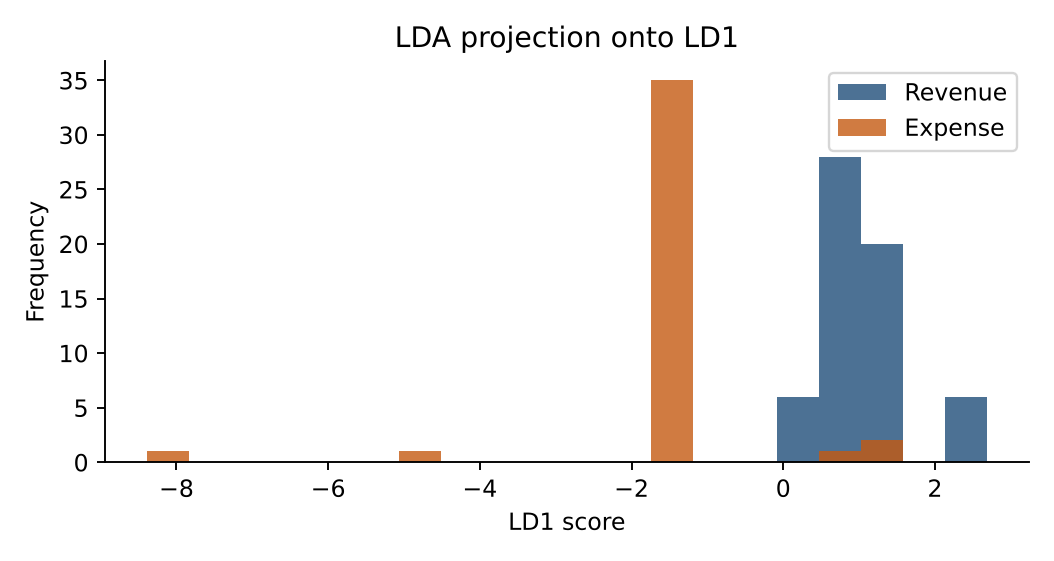
\includegraphics[width=0.68\textwidth]{figures/lda_projection.png}
\caption{LDA projection of revenue and expense transactions.}
\sourcecaption
\end{figure}

\subsection{Linear regression}
Ordinary least squares models transaction amount as a function of day index. The simple model is $y_i=\beta_0+\beta_1x_i+\epsilon_i$, with estimate
\begin{equation}
  \hat{\boldsymbol{\beta}}=(X^{\mathsf T}X)^{-1}X^{\mathsf T}y.
\end{equation}
The simple model's fitted slope is about INR 556 per day. On the reported test set, the time-only model had $R^2=0.887$, RMSE INR 1,329 and MAE INR 1,192. A multiple model adding expense status and GST rate had test $R^2=0.863$, RMSE INR 1,461 and MAE INR 1,019. These measures answer different error questions; the lower MAE for the multiple model does not mean it has the higher $R^2$.

\begin{table}[H]
\centering
\caption{Regression test-set results}
\begin{tabular}{lrrr}
\toprule
Model & Test $R^2$ & RMSE (INR) & MAE (INR)\\
\midrule
Amount $\sim$ day index & 0.887 & 1,329 & 1,192\\
Amount $\sim$ day index + expense status + GST rate & 0.863 & 1,461 & 1,019\\
\bottomrule
\end{tabular}
\end{table}

\begin{figure}[H]
\centering
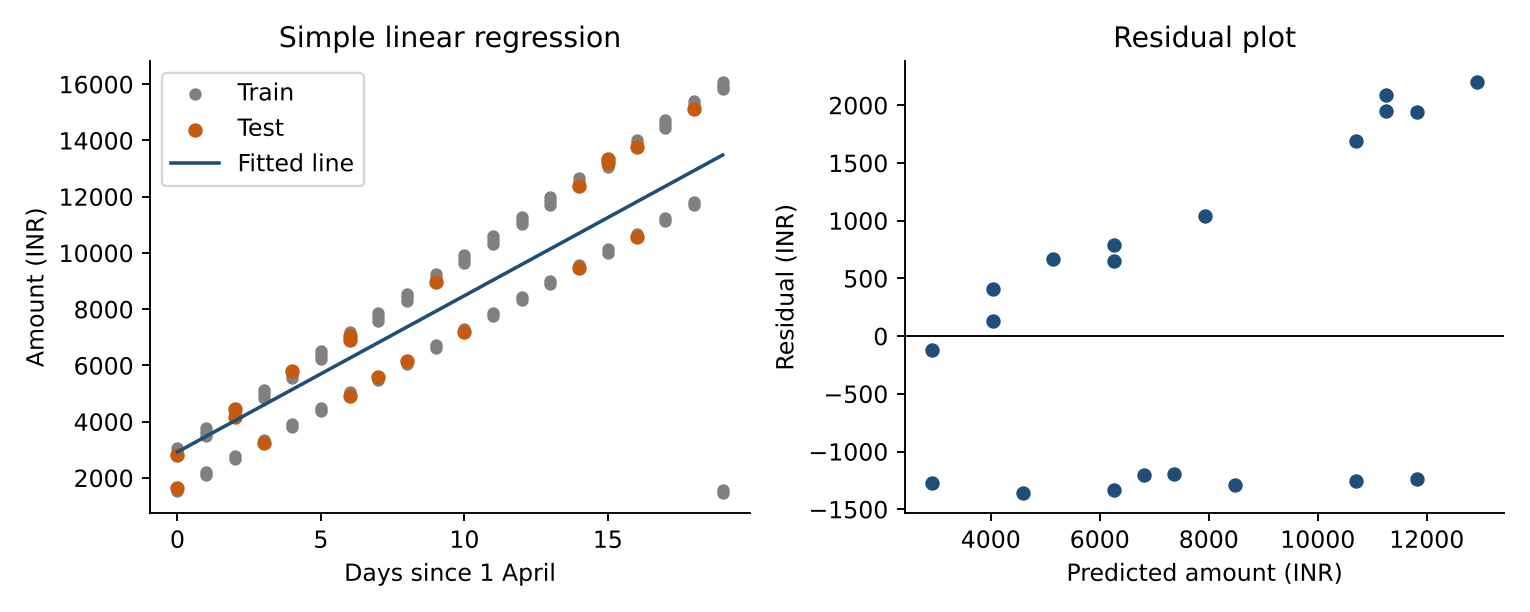
\includegraphics[width=0.88\textwidth]{figures/regression_fit_and_residuals.png}
\caption{Simple regression fit and residuals. The residual bands reflect revenue and expense records with different amount patterns.}
\sourcecaption
\end{figure}

\clearpage
\section{Findings, limitations and conclusion}
The results answer the project objectives: cleaning corrected 17 net amount errors; descriptive statistics summarized transaction flows; hypothesis tests found a difference between revenue and expense transaction means and a strong GST-rate association with transaction type; PCA retained 85.2\% of variance in two components; LDA separated the labels in this sample; and regression captured the increasing amount pattern over the 20-day period.

The findings are limited by the 100-row sample, its single-hotel and 20-day scope, and the project documentation's description of the data as generated. Several features are structurally related to transaction type, so LDA performance may be optimistic. Payment mode is confounded with transaction type. Department mismatches and zero-rate GST records also limit financial interpretation. Numeric treatment of account codes in PCA may impose an artificial order on categories.

The analysis demonstrates a practical data science workflow, but it does not establish that the observed pattern will continue in a real hotel. Further work should use validated multi-month operating data, reconcile department and account coding at source, add occupancy and seasonal variables, and evaluate models on a later time period.

\subsection{Repository and demonstration}
The project repository is available at \url{https://github.com/Ishavijay/Fds-project--lab-work-}. A clear demonstration can load the prepared workbook, show the 17 corrected net values, summarize revenue and expenses, explain one hypothesis test, then display PCA, LDA and regression results with their limitations. The supplied materials did not include an Overleaf project URL; the LaTeX source and figure files are included with this report.

\begin{thebibliography}{9}
\bibitem{projectreport}
I. Vijay, S. Chitra and S. Singhal, \textit{Hotel Accounts Analysis and Transaction Prediction: Project Documentation}, supplied project report, n.d.

\bibitem{dataset}
\textit{Hotel Accounts Analysis-Ready Workbook}, supplied Excel dataset, 100 transactions, April 2025.

\bibitem{description}
\textit{Data Description -- Hotel Accounts}, supplied dataset documentation, n.d.

\bibitem{rubric}
\textit{Fundamentals of Data Science -- Project Assessment Rubric}, supplied course assessment document, n.d.
\end{thebibliography}

\end{document}
